\documentclass[tikz,border=10pt]{standalone}
\usepackage{tikz}
\usetikzlibrary{shapes.geometric,arrows.meta,positioning,fit,backgrounds,shadows.blur}

\definecolor{greenFill}{HTML}{E8F5E9}
\definecolor{greenStroke}{HTML}{43A047}
\definecolor{memFill}{HTML}{FFF3E0}
\definecolor{memStroke}{HTML}{FFB74D}
\definecolor{coreFill}{HTML}{E1F5FE}
\definecolor{coreStroke}{HTML}{0277BD}
\definecolor{optFill}{HTML}{FCE4EC}
\definecolor{optStroke}{HTML}{E91E63}
\definecolor{procFill}{HTML}{FFF9C4}
\definecolor{procStroke}{HTML}{FBC02D}
\definecolor{textMain}{HTML}{263238}
\definecolor{textMuted}{HTML}{607D8B}

\begin{document}
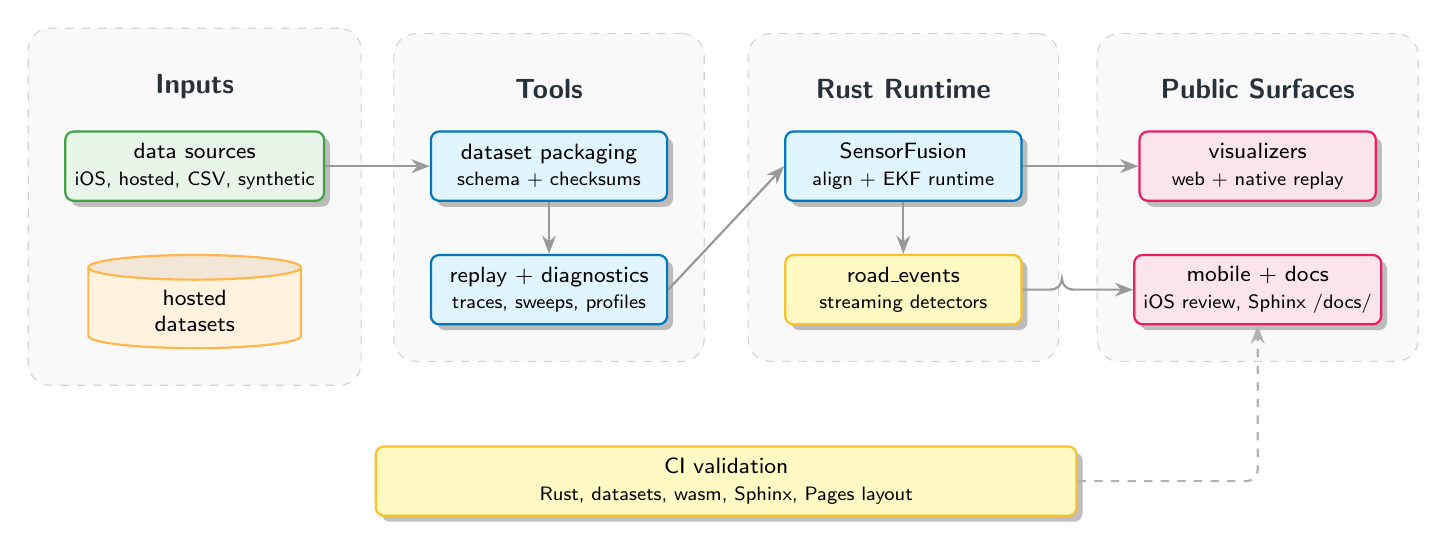
\begin{tikzpicture}[
    node distance=0.66cm and 1.45cm,
    font=\sffamily\footnotesize,
    >=Stealth,
    dataNode/.style={
        rectangle, rounded corners=3pt,
        draw=greenStroke, thick,
        fill=greenFill,
        minimum width=3.0cm, minimum height=0.88cm,
        align=center,
        drop shadow
    },
    memNode/.style={
        cylinder, cylinder uses custom fill,
        cylinder body fill=memFill, cylinder end fill=memFill!90!gray,
        shape border rotate=90,
        aspect=0.25,
        draw=memStroke, thick,
        minimum width=2.7cm, minimum height=1.0cm,
        align=center
    },
    opNode/.style={
        rectangle, rounded corners=3pt,
        draw=coreStroke, thick,
        fill=coreFill,
        minimum width=3.0cm, minimum height=0.88cm,
        align=center,
        drop shadow
    },
    procNode/.style={
        rectangle, rounded corners=3pt,
        draw=procStroke, thick,
        fill=procFill,
        minimum width=3.0cm, minimum height=0.88cm,
        align=center,
        drop shadow
    },
    optNode/.style={
        rectangle, rounded corners=3pt,
        draw=optStroke, thick,
        fill=optFill,
        minimum width=3.0cm, minimum height=0.88cm,
        align=center,
        drop shadow
    },
    group/.style={
        draw=gray!35, dashed, rounded corners=8pt,
        inner sep=13pt, fill=gray!5
    },
    title/.style={font=\sffamily\bfseries, text=textMain, align=center},
    note/.style={font=\scriptsize, text=textMuted, align=center},
    flow/.style={->, thick, draw=gray!80, rounded corners=4pt},
    support/.style={->, thick, dashed, draw=gray!60, rounded corners=4pt}
]

% Layout plan: one dominant left-to-right path with only one secondary CI path.
\node[dataNode] (Sources) at (0, 1.0)
  {data sources\\\scriptsize iOS, hosted, CSV, synthetic};
\node[memNode, below=of Sources] (Datasets) {hosted\\datasets};
\node[title, above=0.28cm of Sources] (InputTitle) {Inputs};

\node[opNode] (Packaging) at (4.5, 1.0)
  {dataset packaging\\\scriptsize schema + checksums};
\node[opNode, below=of Packaging] (Replay) {replay + diagnostics\\\scriptsize traces, sweeps, profiles};
\node[title, above=0.28cm of Packaging] (ToolTitle) {Tools};

\node[opNode] (Fusion) at (9.0, 1.0)
  {SensorFusion\\\scriptsize align + EKF runtime};
\node[procNode, below=of Fusion] (Events) {road\_events\\\scriptsize streaming detectors};
\node[title, above=0.28cm of Fusion] (RuntimeTitle) {Rust Runtime};

\node[optNode] (Visualizer) at (13.5, 1.0)
  {visualizers\\\scriptsize web + native replay};
\node[optNode, below=of Visualizer] (Mobile) {mobile + docs\\\scriptsize iOS review, Sphinx /docs/};
\node[title, above=0.28cm of Visualizer] (SurfaceTitle) {Public Surfaces};

\node[procNode, minimum width=8.9cm] (CI) at (6.75, -3.0)
  {CI validation\\\scriptsize Rust, datasets, wasm, Sphinx, Pages layout};

\begin{scope}[on background layer]
  \node[group, fit=(InputTitle)(Sources)(Datasets)] {};
  \node[group, fit=(ToolTitle)(Packaging)(Replay)] {};
  \node[group, fit=(RuntimeTitle)(Fusion)(Events)] {};
  \node[group, fit=(SurfaceTitle)(Visualizer)(Mobile)] {};
\end{scope}

\draw[flow] (Sources.east) -- (Packaging.west);
\draw[flow] (Packaging.south) -- (Replay.north);
\draw[flow] (Replay.east) -- (Fusion.west);
\draw[flow] (Fusion.south) -- (Events.north);
\draw[flow] (Fusion.east) -- (Visualizer.west);
\draw[flow] (Events.east) -- ++(0.5,0) |- (Mobile.west);
\draw[support] (CI.east) -| (Mobile.south);

\end{tikzpicture}
\end{document}
